\begin{figure*}[t]
	\centering
	\addtolength{\tabcolsep}{-4.5pt}
	\begin{tabular}{ccccccccc}
		\raisebox{20pt}{\rotatebox{90}{\small Photo}}
		&
		\begin{overpic}[width=\resultwidth]{real/bump_1/target.jpg}
			\imglabeltop{Bump-3}
		\end{overpic}
		&
		\begin{overpic}[width=\resultwidth]{real/leather_1/target.jpg}
			\imglabeltop{Leather-3}
		\end{overpic}
		&
		\begin{overpic}[width=\resultwidth]{real/leather_4/target.jpg}
			\imglabeltop{Leather-6}
		\end{overpic}
		&
		\begin{overpic}[width=\resultwidth]{real/plaster_1/target.jpg}
			\imglabeltop{Plaster-3}
		\end{overpic}
		&
		\begin{overpic}[width=\resultwidth]{real/flake_2/target.jpg}
			\imglabeltop{Metallicflake-4}
		\end{overpic}
		&
		\begin{overpic}[width=\resultwidth]{real/metal_1/target.jpg}
			\imglabeltop{Brushmetal-3}
		\end{overpic}
		&
		\begin{overpic}[width=\resultwidth]{real/wood_1/target.jpg}
			\imglabeltop{Wood-3}
		\end{overpic}
		&
		\begin{overpic}[width=\resultwidth]{real/wood_2/target.jpg}
			\imglabeltop{Wood-4}
		\end{overpic}
		\\
		\raisebox{20pt}{\rotatebox{90}{\small Ours}} &
		\includegraphics[width=\resultwidth]{real/bump_1/good1.jpg} &
		\includegraphics[width=\resultwidth]{real/leather_1/good1.jpg} &
		\includegraphics[width=\resultwidth]{real/leather_4/good1.jpg} &
		\includegraphics[width=\resultwidth]{real/plaster_1/good1.jpg} &
		\includegraphics[width=\resultwidth]{real/flake_2/good1.jpg} &
		\includegraphics[width=\resultwidth]{real/metal_1/good1.jpg} &
		\includegraphics[width=\resultwidth]{real/wood_1/good1.jpg} &
		\includegraphics[width=\resultwidth]{real/wood_2/good1.jpg}
		\\
		\raisebox{10pt}{\rotatebox{90}{\small \cite{Hu2019}}} &
		\includegraphics[width=\resultwidth]{Hu/bump3.jpg} &
		\includegraphics[width=\resultwidth]{Hu/leather3.jpg} &
		\includegraphics[width=\resultwidth]{Hu/leather6.jpg} &
		\includegraphics[width=\resultwidth]{Hu/plaster3.jpg} &
		\includegraphics[width=\resultwidth]{Hu/flake4.jpg} &
		\includegraphics[width=\resultwidth]{Hu/metal3.jpg} &
		\includegraphics[width=\resultwidth]{Hu/wood3.jpg} &
		\includegraphics[width=\resultwidth]{Hu/wood4.jpg}
	\end{tabular}
	\captionsetup{labelfont=bf,textfont=it}
	\caption{\label{fig:Hu}
		\textbf{Comparison} to the forward neural prediction method of Hu et al. \cite{Hu2019}, where we apply their network structure with our BRDFs and lighting conditions. The photo (top) is better matched by our MCMC sampling results (middle) than their prediction (bottom), which moreover tends to become worse for more complex BRDF models and with more parameters. On the other hand, \cite{Hu2019} can be used as an efficient initialization of our sampling, as shown in Figure \ref{fig:Hu2}.
	}
\end{figure*}

\begin{figure}[t]
	\centering
	\addtolength{\tabcolsep}{-3pt}
	\begin{tabular}{cccc}
		%		 &
		%		\raisebox{0pt}{\includegraphics[width=0.32\columnwidth]{img/sample1_200.pdf}} &
		%		\raisebox{0pt}{\includegraphics[width=0.32\columnwidth]{img/sample2_200.pdf}} &
		%		\raisebox{30pt}{\rotatebox{90}{$N=200$}} \\
		\raisebox{10pt}{
\includegraphics[width=0.25\columnwidth]{init/target.jpg}} &
		\raisebox{-4pt}{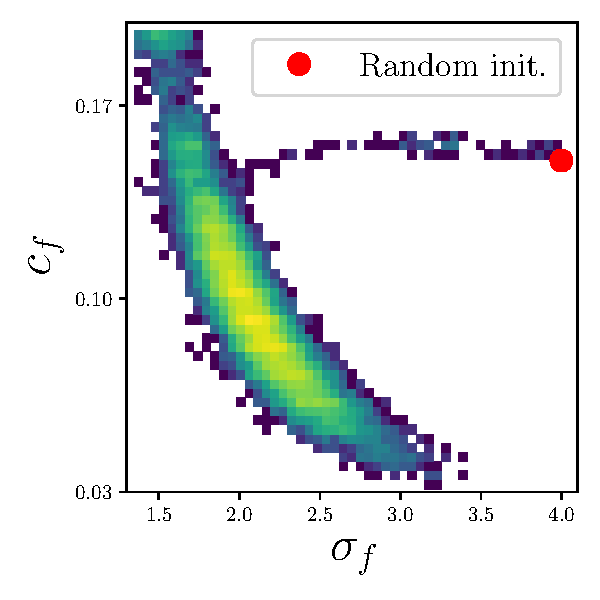
\includegraphics[width=0.32\columnwidth]{init/sample1.pdf}} &
		\raisebox{-4pt}{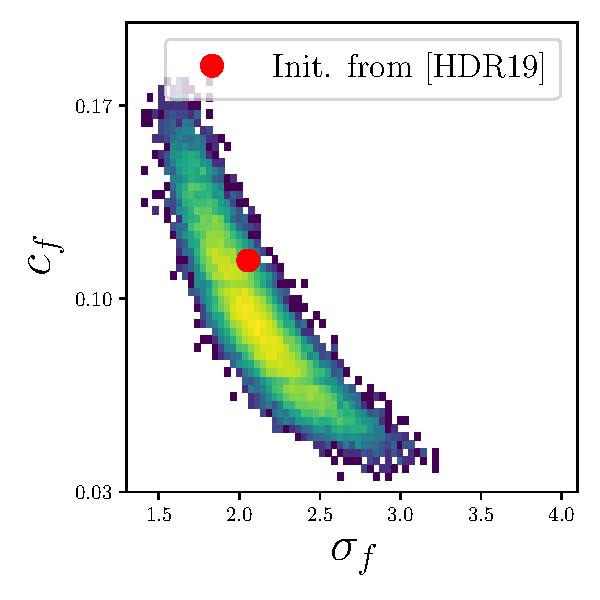
\includegraphics[width=0.32\columnwidth]{init/sample2.pdf}} &
		\raisebox{16pt}{\rotatebox{90}{$N=22500$}} \\
		Target & (a) & (b)
	\end{tabular}
	\captionsetup{labelfont=bf,textfont=it}
	\caption{\label{fig:Hu2}
		\textbf{Initialization} of our sampling with the method of Hu et al. \cite{Hu2019} on a synthetic bumpy surface example. The figure shows joint posterior distributions over two parameters using different initializations: a random initialization drawn from the prior (a) and the prediction of \cite{Hu2019} (b). As we can see, starting from the result of \cite{Hu2019} can shorten the burn-in phase of the MCMC sampling process.
	}
\end{figure}
